% chapter 4 section 1

\section{电场}

\subsection{电场}

\subsubsection{电荷}

物体的带电量称为电荷,日文中也可用電気量一词。其单位为库伦(C),且带电体间时常有满足库仑定律\footnote{诱电率$\varepsilon=\frac{1}{4k\pi}$}的作用力存在。
\begin{itembox}[l]{库仑定律}
    \begin{equation*}
        F=k\frac{Qq}{r^2}
    \end{equation*}
    \begin{itemize}
        \item $k=9\times10^9N\cdot m^2\cdot C^{-2}$
        \item 同性相斥,异性相吸
    \end{itemize}
\end{itembox}

\subsubsection{电场}

为了更方便得解释诸如重力、万有引力、电磁力等非接触力的作用方式,人们引入了“场” 的概念,并认为是场传递了各种各样的物理信息。因此在空间中传递上述库仑力的场即为\underline{电场},用单位电荷的受力定义。

\begin{figure}[p!]
    \centering
    \begin{minipage}[t]{0.48\textwidth}
        \centering
        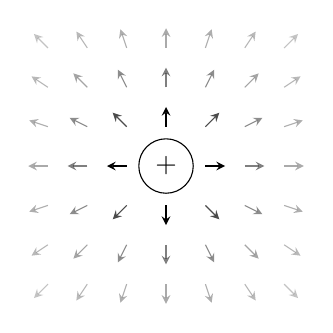
\begin{tikzpicture}[scale=0.5]
            \node[draw, circle] at (0,0) {$+$};
            \foreach \x in {-3,...,3} \foreach \y in {-3,...,3} {
                \pgfmathparse{and(equal(\x,0),equal(\y,0))}
                \ifnum\pgfmathresult=1
                \else
                \draw[-stealth, opacity={1/sqrt((\x)^2+(\y)^2)}] (\x,\y) -- ++ (
                    {0.5*\x/sqrt((\x)^2+(\y)^2)},
                    {0.5*\y/sqrt((\x)^2+(\y)^2)}
                );
                \fi
            }
        \end{tikzpicture}
        \caption{单正点电荷电场图示}
    \end{minipage}
    \begin{minipage}[t]{0.48\textwidth}
        \centering
        \begin{tikzpicture}[scale=0.5]
            \node[draw, circle] at (0,0) {$-$};
            \foreach \x in {-3,...,3} \foreach \y in {-3,...,3} {
                \pgfmathparse{and(equal(\x,0),equal(\y,0))}
                \ifnum\pgfmathresult=1
                \else
                \draw[-stealth, opacity={1/sqrt((\x)^2+(\y)^2)}] ($(\x,\y)+(
                    {0.5*\x/sqrt((\x)^2+(\y)^2)},
                    {0.5*\y/sqrt((\x)^2+(\y)^2)}
                )$) -- (\x,\y);
                \fi
            }
        \end{tikzpicture}
        \caption{单负点电荷电场图示}
    \end{minipage}
\end{figure}

\begin{figure}[p!]
    \centering
    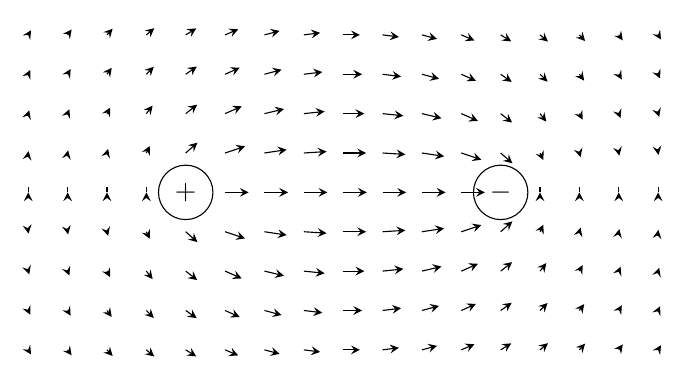
\begin{tikzpicture}[scale=0.5]
        \node[draw, circle] at (-4,0) {$+$};
        \node[draw, circle] at (4,0) {$-$};
        \foreach \x in {-8,...,8} \foreach \y in {-4,...,4} {
            \pgfmathparse{or(
                and(equal(\x,-4),equal(\y,0)),
                and(equal(\x,4),equal(\y,0))
            )}
            \ifnum\pgfmathresult=1
            \else
            \draw[-stealth] (\x,\y) -- ++ (
                {0.3*((\x+4)/sqrt((\x+4)^2+(\y)^2)-(\x-4)/sqrt((\x-4)^2+(\y)^2))},
                {0.3*(\y/sqrt((\x+4)^2+(\y)^2)-\y/sqrt((\x-4)^2+(\y)^2))}
            );
            \fi
        }
    \end{tikzpicture}
    \caption{正-负点电荷电场图示}
\end{figure}

\begin{figure}[p!]
    \centering
    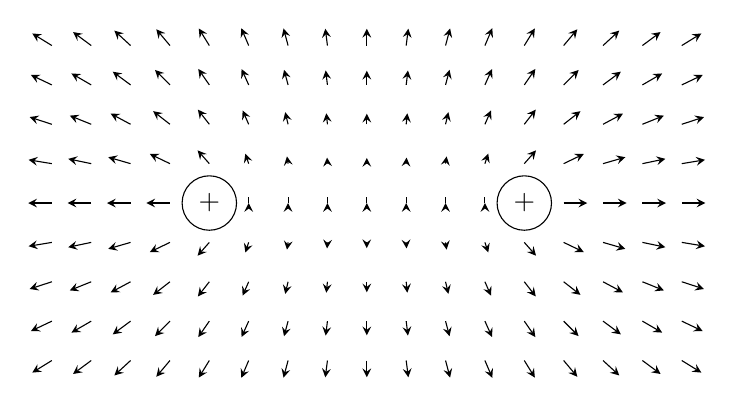
\begin{tikzpicture}[scale=0.5]
        \node[draw, circle] at (-4,0) {$+$};
        \node[draw, circle] at (4,0) {$+$};
        \foreach \x in {-8,...,8} \foreach \y in {-4,...,4} {
            \pgfmathparse{or(
                and(equal(\x,-4),equal(\y,0)),
                and(equal(\x,4),equal(\y,0))
            )}
            \ifnum\pgfmathresult=1
            \else
            \draw[-stealth] (\x,\y) -- ++ (
                {0.3*((\x+4)/sqrt((\x+4)^2+(\y)^2)+(\x-4)/sqrt((\x-4)^2+(\y)^2))},
                {0.3*(\y/sqrt((\x+4)^2+(\y)^2)+\y/sqrt((\x-4)^2+(\y)^2))}
            );
            \fi
        }
    \end{tikzpicture}
    \caption{正-正点电荷电场图示}
\end{figure}

\begin{itembox}[l]{电场}
    \begin{equation*}
        \vec{E}=\frac{\vec{F}}{q}
        \iff
        \vec{F}=q\vec{E}
    \end{equation*}
    \begin{itemize}
        \item 单位:N/C
        \item 点电荷周围的电场:$E=k\frac{Q}{r^2}$
    \end{itemize}
\end{itembox}
根据定义可知电场也是一个矢量,所以在实际运用过程中也满足矢量的合成与分解。

\subsection{电势}

\subsubsection{电势能与电势}

观察库仑力形式可发现其与万有引力十分相像,因此不难推测库仑力也是保存力。因而也有其对应的势能,即\underline{电势能},日文为静電気力による位置エネルギー。

此外,为了描述物理现象与计算使用方便,人们也引入了电场中单位电荷的电势能:电势(日文为電位)这个物理量,单位为伏特(V)。因此,电势能与电势之间满足如下关系。
\begin{itembox}[l]{电势能与电势}
    \begin{equation*}
        U=qV
    \end{equation*}
\end{itembox}

\subsubsection{典型电场中的电势}

\paragraph{匀强电场的电势}日文为一様電場,即大小、方向均衡定的电场。
\begin{figure}[ht!]
    \centering
    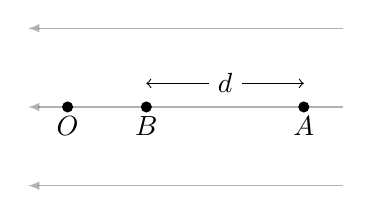
\begin{tikzpicture}
        \foreach \y in {0,1,2} {\draw[opacity=0.3, -latex] (4,\y) -- (0,\y);}
        \fill (0.5,1) circle (2pt) node[below] {$O$};
        \fill (1.5,1) circle (2pt) node[below] {$B$};
        \fill (3.5,1) circle (2pt) node[below] {$A$};
        \draw[<->] (1.5,1.3) -- node[fill=white] {$d$} (3.5,1.3);
    \end{tikzpicture}
    \caption{匀强电场电势}
\end{figure}
那么,匀强电场中倘若某两点间距为$d$,期间将会存在
\begin{equation*}
    V=\frac{Eq\times d}{q}=Ed
\end{equation*}
大小的电势,并称其为该两点间的\underline{电势差}。

\paragraph{点电荷电场的电势}

规定离场源电荷无限远处为电势基准,则可得点电荷周围电势公式。
\begin{itembox}[l]{点电荷电势}
    \begin{equation*}
        U=k\frac{Q}{r}
    \end{equation*}
\end{itembox}

\subsubsection{等电势面}

类比于地图上描述地势分布的等高线,等电势线/面也常常用于描述电势的分布,且具有如下性质。
\begin{itemize}
    \item 与电场线垂直
    \item 等电位面密$\iff$电场线密$\iff$电场强
\end{itemize}
\begin{figure}[ht!]
    \centering
    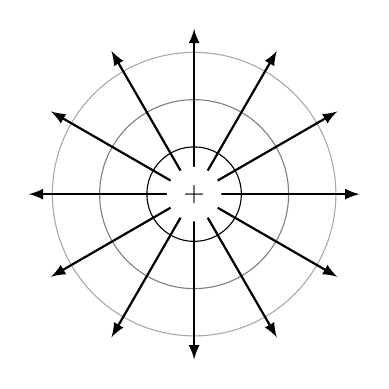
\begin{tikzpicture}[scale=0.6]
        \foreach \r in {1,...,3} {\draw[opacity={1/\r}] (0,0) circle (\r);}
        \foreach \a in {1,...,12} {\draw[thick, -latex] (0,0) -- ({\a*30}:3.5);}
        \node[circle, fill=white] at (0,0) {$+$};
    \end{tikzpicture}
    \caption{等电势面}
\end{figure}

\subsubsection{总结}

鉴于本节内容较多且不易梳理清晰,特此简做总结。
\begin{figure}[ht!]
    \centering
    \renewcommand\arraystretch{1.5}
    \begin{tabular}{c|c|c|c|c}
        \hline
        &电场E&库仑力F&电势能U&电势V\\\hline
        重力场&$g$&$mg$&$mgh$&$gh$\\\hline
        点电荷&$\frac{kQ}{r^2}$&$\frac{kQq}{r^2}$&$\frac{kQq}{r}$&$\frac{kQ}{r}$\\\hline
    \end{tabular}
    \caption{电场电势总结}
\end{figure}

\subsection{电容器}

\subsubsection{基本原理}

电容器,日文为コンデンサー,是电路中基本的储能元件,其符号如图。
\begin{figure}[ht!]
    \centering
    \begin{circuitikz}
        \draw (0,0) to[C=$3\mu F$,o-o] (2,0);
    \end{circuitikz}
\end{figure}
就比较简单的平行板电容器而言,其基本工作原理为:极板两端由于电势高低不同因而汇聚正负电荷,异种电荷相互吸引从而不断增大极板两端的电势差,直到与外路相同为止。在这个过程中电容器所“收集”的电荷量可由电容器定义式得来。
\begin{itembox}[l]{电容器定义式}
    \begin{equation*}
        Q=CV
    \end{equation*}
    \begin{itemize}
        \item V:极板两端的电势差
        \item C:电容量,日文为電気容量,单位为法拉(F)
    \end{itemize}
\end{itembox}

\begin{itembox}[l]{平行板电容器}
    \begin{equation*}
        C=\varepsilon_0\frac{S}{d}
    \end{equation*}
    \begin{itemize}
        \item $\varepsilon_0$:绝对诱电率
        \item 极板间电场:$E=\frac{V}{d}=\frac{Q}{\varepsilon_0S}$
    \end{itemize}
\end{itembox}

\subsubsection{电容器串并联}

\begin{figure}[ht!]
    \centering
    \begin{minipage}{0.48\textwidth}
        \begin{itembox}[l]{串联}
            \begin{itemize}
                \item 电荷相等
                \item $\frac{Q}{C_1}+\frac{Q}{C_2}=V$
                \item $\frac{Q}{C}=V$
                \item $\frac{1}{C}=\frac{1}{C_1}+\frac{1}{C_2}$
            \end{itemize}
        \end{itembox}
    \end{minipage}
    \begin{minipage}{0.48\textwidth}
        \centering
        \begin{circuitikz}[european]
            \draw (0,0)
            to[battery1, invert] (0,2)
            to[short] (2,2)
            to[C=$C_1$] (2,1)
            to[C=$C_2$] (2,0)
            to[short] (0,0);
        \end{circuitikz}
        \caption{电容器串联}
    \end{minipage}
\end{figure}

\begin{figure}[ht!]
    \centering
    \begin{minipage}{0.48\textwidth}
        \begin{itembox}[l]{并联}
            \begin{itemize}
                \item 电压相等
                \item $VC_1+VC_2=Q$
                \item $VC=Q$
                \item $C=C_1+C_2$
            \end{itemize}
        \end{itembox}
    \end{minipage}
    \begin{minipage}{0.48\textwidth}
        \centering
        \begin{circuitikz}[european]
            \draw (0,0)
            to[battery1, invert] (0,2)
            to[short] (1.5,2)
            to[C=$C_1$] (1.5,0)
            to[short] (0,0);
            \draw (1.5,2)
            to[short] (3,2)
            to[C=$C_2$] (3,0)
            to[short] (1.5,0);
        \end{circuitikz}
        \caption{电容器并联}
    \end{minipage}
\end{figure}

\subsubsection{电容器储能}

\paragraph{储能}电容器在充电(积攒能量)的过程中,电荷量与电势差共同增长。根据电势能公式,在电势差为V的某个时刻汇聚过来的电荷q会携带$U=qV$大小的能量。将整个过程绘制成$Q-V$图像,那么总能量即为图中三角形的面积。
\begin{figure}[ht!]
    \centering
    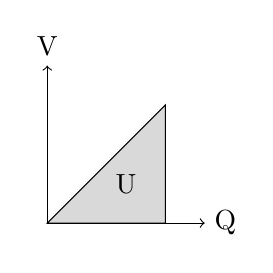
\begin{tikzpicture}
        \draw[->] (0,0) -- (2,0) node[right] {Q};
        \draw[->] (0,0) -- (0,2) node[above] {V};
        \filldraw[color=black, fill=gray, fill opacity=0.3] (0,0) -- (1.5,1.5) -- (1.5,0) -- cycle;
        \node at (1,0.5) {U};
    \end{tikzpicture}
    \caption{电容器储能}
\end{figure}
\begin{itembox}[l]{电容器储能}
    \begin{equation*}
        U=\frac12QV=\frac12CV^2=\frac{Q^2}{2C}
    \end{equation*}
\end{itembox}

此外,假设与电容器串联的外路的总电阻为$R$,那么根据基尔霍夫定律可得
\begin{gather*}
    E=IR+\frac{Q}{C}\\
    I=\frac{E-\frac{Q}{C}}{R}
\end{gather*}
当电路接通的瞬间,电容器不带电($Q=0$),所以回路电流为$I=\frac{E}{R}$。如此一来则可以粗略地认为此时电容器就是一根导线。
\begin{figure}[ht!]
    \centering
    \begin{minipage}{0.48\textwidth}
        \centering
        \begin{tikzpicture}
            \draw[->] (0,0) -- (4,0) node[right] {$t$};
            \draw[->] (0,-1.5) -- (0,1.5) node[above] {$I$};
            \draw[thick] (0,0) -- (0.5,0) -- (0.5,1);
            \draw[thick, domain=0.5:2.5] plot[smooth] (\x, {exp(2-4*\x)});
            \draw[thick] (2.5,0) -- (2.5,-1);
            \draw[thick, domain=2.5:4] plot[smooth] (\x, {-exp(10-4*\x)});
        \end{tikzpicture}
    \end{minipage}
    \begin{minipage}{0.48\textwidth}
        \centering
        \begin{tikzpicture}
            \draw[->] (0,0) -- (4,0) node[right] {$t$};
            \draw[->] (0,-1.5) -- (0,1.5) node[above] {$V$};
            \draw[thick] (0,0) -- (0.5,0);
            \draw[thick, domain=0.5:2.5] plot[smooth] (\x, {1-exp(2-4*\x)});
            \draw[thick, domain=2.5:4] plot[smooth] (\x, {exp(10-4*\x)});
        \end{tikzpicture}
    \end{minipage}
    \caption{电容器储能时IV变化}
\end{figure}

\paragraph{损耗}在给电容器充电的过程中,电源做功\footnote{给$Q$大小的电荷提供了$V$大小的电压,使其获得了$QV$大小的电势能}为$W=QV$。根据能量守恒定律可知,其中有
\begin{equation*}
    W-U=QV-\frac12QV=\frac12QV
\end{equation*}
大小的能量在途中损耗了。由于整个过程中没有其他能量形式,因此可知整个充电过程中产生了$\frac12QV$大小的焦耳热。

\subsubsection{极板间引力}

结合带电体在电场中的受力可知,平行板电容器的极板间存在相互吸引的力。其间的电场为$E=E_\textrm{上}+E_\textrm{下}$,因为上下极板带电量相等,所以产生的场强也相等。着眼于上极板吸引下极板的部分可得
\begin{itembox}[l]{极板间引力}
    \begin{equation*}
        F=QE_\textrm{上}=\frac12QE
    \end{equation*}
\end{itembox}

\subsubsection{平行板电容器改装}

\begin{figure}[ht!]
    \centering
    \begin{minipage}[t]{0.48\textwidth}
        \centering
        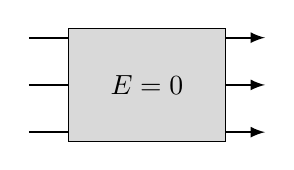
\begin{tikzpicture}[yscale=0.6]
            \foreach \y in {0,1,2} {\draw[thick, -latex] (0,\y) -- (3,\y);}
            \filldraw[color=black, fill=gray!30] (0.5,-0.2) rectangle (2.5,2.2);
            \node at (1.5,1) {$E=0$};
        \end{tikzpicture}
        \caption{静电屏蔽}
    \end{minipage}
    \begin{minipage}[t]{0.48\textwidth}
        \centering
        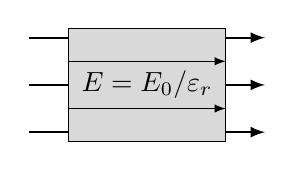
\begin{tikzpicture}[yscale=0.6]
            \foreach \y in {0,1,2} {\draw[thick, -latex] (0,\y) -- (3,\y);}
            \filldraw[color=black, fill=gray!30] (0.5,-0.2) rectangle (2.5,2.2);
            \foreach \y in {0.5,1.5} {\draw[-latex] (0.5,\y) -- (2.5,\y);}
            \node at (1.5,1) {$E=E_0/\varepsilon_r$};
        \end{tikzpicture}
        \caption{电极化}
    \end{minipage}
\end{figure}

\paragraph{静电屏蔽}日文为静電遮蔽。将导体放入电场后,导体中的电子受电场力影响汇聚到导体两端,形成抵消外部电场的电场。

\paragraph{电极化}日文为誘電分極。将绝缘体放入电场后,由于内部电子无法自由移动,只能发生小范围偏移,因而无法完全抵消外部电场。所以在日文中绝缘体也可称作誘電体。

\begin{figure}[ht!]
    \centering
    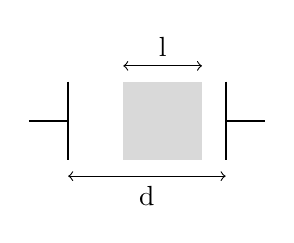
\begin{tikzpicture}
        \draw[thick] (0,0) -- (0.5,0);
        \draw[thick] (2.5,0) -- (3,0);
        \draw[thick] (0.5,0.5) -- (0.5,-0.5);
        \draw[thick] (2.5,0.5) -- (2.5,-0.5);
        \fill[fill=gray!30] (1.2,-0.5) rectangle (2.2,0.5);
        
        \draw[<->] (1.2,0.7) -- node[above] {l} (2.2,0.7);
        \draw[<->] (0.5,-0.7) -- node[below] {d} (2.5,-0.7);
    \end{tikzpicture}
    \caption{电容器改装}
\end{figure}

\paragraph{导体改装}根据静电屏蔽现象可知导体块内无电场,因此没有电势降落,所以可以视其为一段导线。现假设插入的导体块与左极板的距离为x,则根据电容器串联公式可得
\begin{gather*}
    \frac{1}{C}=\frac{1}{\varepsilon_0\frac{S}{x}}+\frac{1}{\varepsilon_0\frac{S}{d-l-x}}\\
    C=\varepsilon_0\frac{S}{d-l}
\end{gather*}

\paragraph{绝缘体改装}主体思路与导体改装一致:将改装后的电容器视作多个电容器串联。在此只补充含绝缘体部分的电容量的变化
\begin{gather*}
    E^\prime=\frac{E}{\varepsilon_r}\implies
    V^\prime=\frac{V}{\varepsilon_r}\\
    Q=CV=C^\prime V^\prime\\
    C^\prime=\varepsilon_rC
\end{gather*}

\paragraph{复杂改装}时而题目中也会出现插入的物体不足以覆盖整个极板的情况,此时只需将已覆盖的部分与未覆盖的部分看作两个电容器并联处理即可。
